\chapter{Erstellung der Computerspielengines}
\label{chapter:erstellung-der-computerspielengines}

TODO:

\section{Ansatz A: Zufallsauswahl der Spielzüge}
\label{section:erstellung-ansatz-a}

TODO:

\begin{itemize}
    \item generelle Player struktur
    \item TODO: add greedy player as another base comparision
\end{itemize}

\lstinputlisting[
    label={code:random-player},
    caption={Definition des RandomPlayers},
    captionpos=b,
    language=Rust,
    firstline=0,
]{res/code/random-player.rs}


\section{Ansatz B: Minimax-Algorithmus}
\label{section:erstellung-ansatz-b}

TODO:

\begin{itemize}
    \item NegaMax-Algorithmus
    \item Principal Variation Search (PVS)
    \item Iterative Deepening
    \item Aspiration Windows
    \item Transposition Table With Zobrist Hashing
    \item Search Extension
    \item Move Ordering
    \item Late Move Reduction
    \item Late Move Pruning
\end{itemize}

\section{Ansatz C: Monte Carlo Tree Search}
\label{section:erstellung-ansatz-c}

TODO:

\begin{itemize}
    \item Normaler MCTS
    \item UCT (Upper Confidence Bound for Trees)
    \item Parallel (Root und Leaf)
    \item Tree Reuse
    \item Evaluator (WinLoss, Score) -> In Eval genauer betrachten
\end{itemize}

\section{Ansatz D: AlphaZero}
\label{section:erstellung-ansatz-d}

TODO:

\begin{itemize}
    \item Grafik von der Netzwerkarchitektur
    \item Parallelization with Virtual Loss
    \item Training-Loop
\end{itemize}

\subsubsection*{Kodierung des Spielzustandes}

\begin{figure}[!ht]
    \centering
    \vspace*{-1.75cm}
    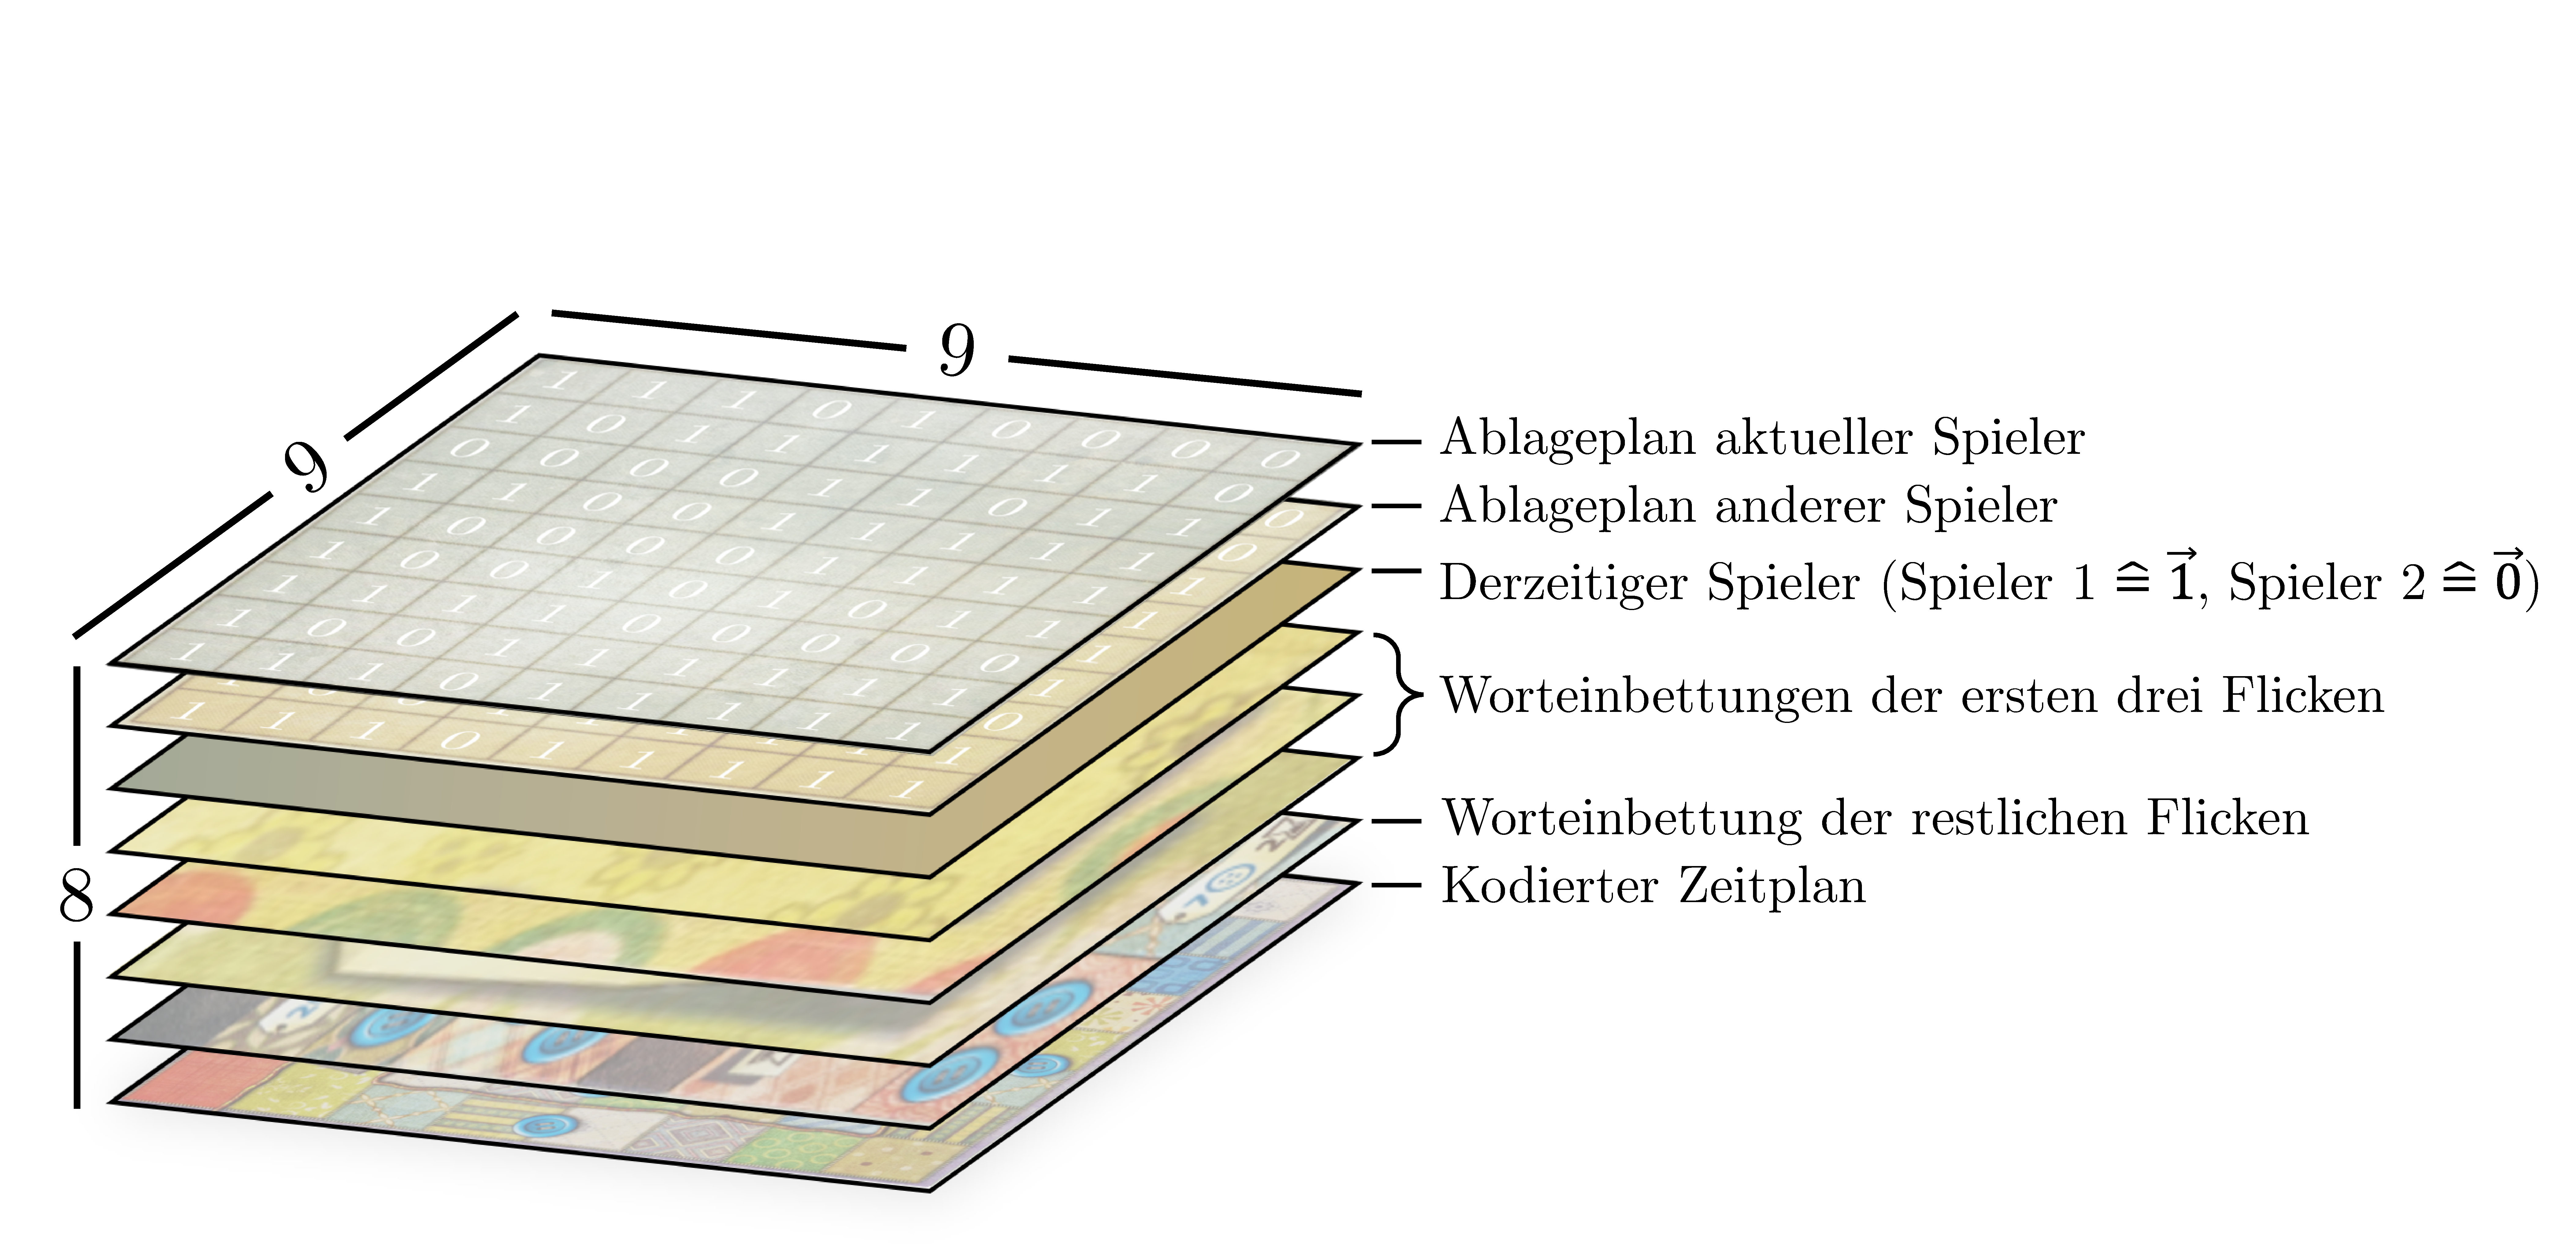
\includegraphics[width=\textwidth]{res/pictures/patch-zero-state.pdf}
    \caption{Zustandskodierung von PatchZero}
    \label{fig:patch-zero-state}
\end{figure}

TODO:

\subsubsection*{Netzwerk-Architektur}

\begin{figure}[!ht]
    \centering
    \vspace*{-1.75cm}
    \includegraphics[width=\textwidth]{res/pictures/patch-zero-architecture.pdf}
    \caption{Architektur von PatchZero}
    \label{fig:patch-zero-architecture}
\end{figure}

TODO:
